\chapter{双分辨率词云可视化}
\label{sec:refinement}

我们从上文讨论的设计选择出发,在基准数据上进行了一些先行的尝试,通过不断迭代明确了双分辨率词云的可视化形式以及相应参数。总体而言,我们的策略是在父级词云布局的基础上,通过区域分割与分层布局获得对应的子级词云布局,再对颜色进行相应的调整,最终以频域滤波的方式获得双分辨率词云(见图~\ref{fig:pipeline})。
\begin{figure}[htbp]
	\centering
	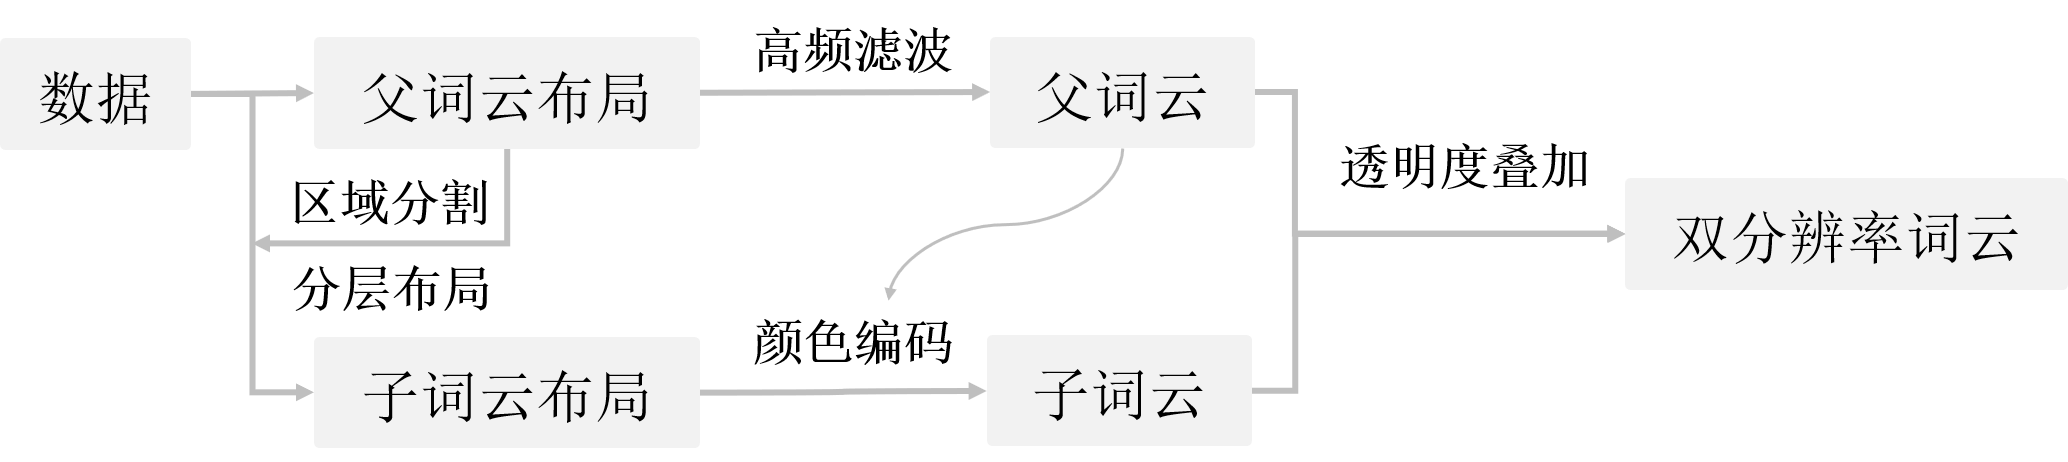
\includegraphics[width=\textwidth]{figures/pipeline.png}
	\caption{多分辨词云生成流程。}
	\label{fig:pipeline}
\end{figure}
\vspace{-1.2cm}

\section{数据}
双分辨率词云的基本数据模型可对应于二分图(见图~\ref{fig:data_model}),父级文本(如关键词,以下简称为父文本)与子级本文(如上下文,以下简称为子文本)之间存在层级的关系或语义上的关联。图中的每一个结点均具有字符串型文本属性和数值型的权重或词频属性(C2)。为了减少数据存储的冗余,使数据简洁而结构明晰,我们选择使用两个序列作为双分辨率词云的表示,分别对应于父文本和子文本,而关联信息编码在父文本各项中。
\begin{figure}[htbp]
	\centering
	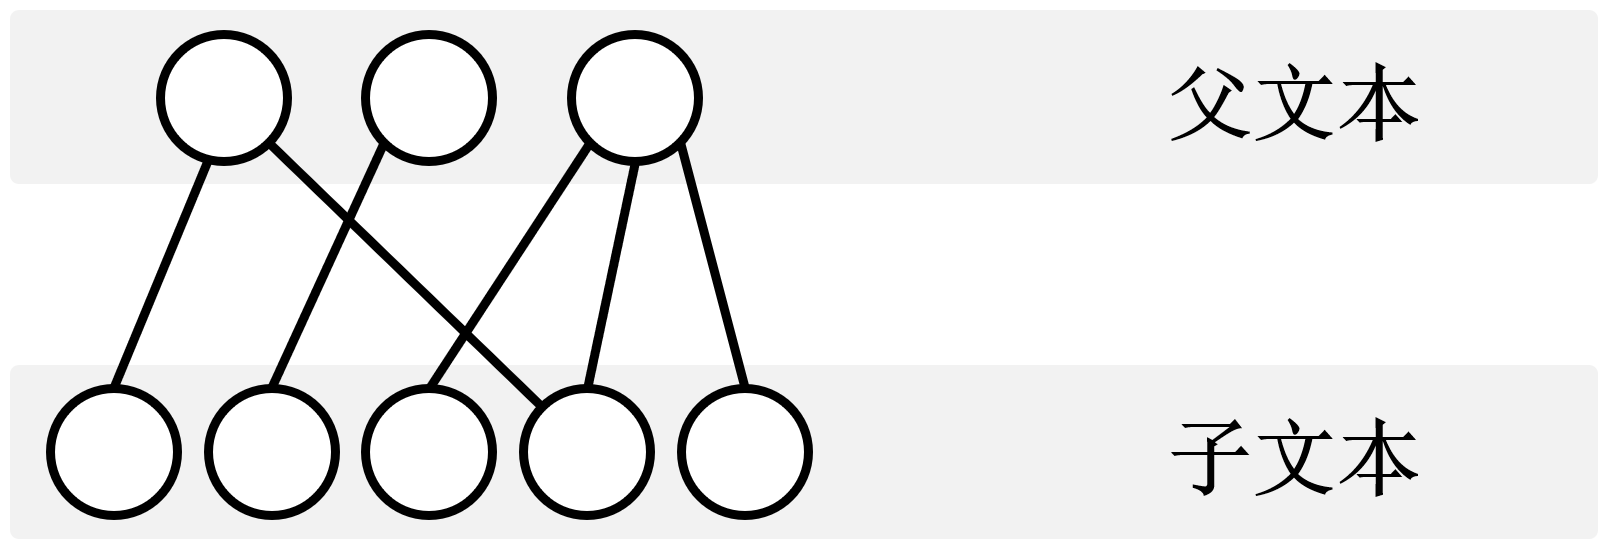
\includegraphics[width=0.6\textwidth]{figures/data_model.png}
	\caption{双分辨率词云数据模型。}
	\label{fig:data_model}
\end{figure}


使用\texttt{YAML}语言,双分辨率词云所对应的数据模型可形式化描述如下。需要注意的是,这里父文本与子文本的权重已归一化。在常见的词云算法中,归一化一般为词频直接除以最大值,亦有取对数或开平方后采用最小-最大归一的方法以降低极端值对整体的影响。

\begin{lstlisting}[language=yaml, caption=数据模型]
# %(*根对象*)
type: object
fileds:
	# %(*contexts域:序列类型,每个对象对应一个上下文*)
	contexts:
		type: sequence
		fields:
			#%(*context域:子文本,上下文*)
			context: { type: string }
			#%(*weight域:子文本权重*)
			weight: { type: number, min: 0, max: 1 }
	# %(*keywords域:序列类型,每个对象对应一个关键词*)
	keywords:
		type: sequence
		fields:
			# %(*keyword域: 父文本,关键词*)
			keyword: { type: string }
			# %(*weight域:关键词权重*)
			weight: { type: number, min: 0, max:1 }
			# %(*contexts域:集合类型,对应的子文本序列号*)
			context:
				type: set
				fields:
					# %(*contextID域:子文本序列号*)
					contextId: { type: number }
\end{lstlisting}

我们选用了《全唐诗》作为探索布局策略的基础数据,提取二字词中词频最高的$30$词作为父文本,对应的诗句(逗号或句号为分句符)作为子文本,并整理为以上数据模型所规定的格式进行尝试。其中,父文本的权重对应于其词频,而子文本的权重对应于该诗句作者在《全唐诗》中被收录的作品数量,在一定程度上通过作者的产量反映诗句的知名度。最终效果可查看图~\ref{fig:tang_poet}。

\section{布局算法}
\label{sec:layout}
我们依次确定父文本词云与子文本词云的位置。其中,父词云由已有词云算法给出,子词云则在对应父元素位置与字形的限制下布局。
\subsection{基础布局}
抽象而言,词云的布局算法就是在给定画布尺寸$w\times h$(长$\times$高)与词集合$\{w_i\}$及其对应字号后$\{s_i\}$,确定每个词在画布上的位置$\{(x_i,\  y_i)\}$,满足在该布局方案下按照给定字号与字体渲染出的词与词之间互不相交即可。

常见的词云算法在第2.3节已有概述,由于它们对不同的分析展示任务各有优势,我们选择在生成双分辨率词云的过程中保留词云布局算法的自由度,用户可根据不同的需求灵活选用适当的布局算法或自定义父词云位置。以下展示了一种最为简单的词云布局算法的伪代码,其主要思想是逐个确定位置,在备选区域中随机选择。
 \begin{algorithm}[htb]
	\caption{适用于轮廓限制的贪心词云布局算法}
	\label{alg:basic_layout}
	\begin{algorithmic}[1]
		\Require
		词云字体$font$;词云对应的文本有序列表$\{(word_i, size_i)\}$,包括文字$word$与字号$size$,顺序为字号由大到小,相同字号按照文字长度由大到小;轮廓限制$Mask$(一般情况下为空白)与其最小外接矩形规格$W\times H$
		\Ensure
		词云布局方案$P$
		\State 基于轮廓限制构建一个二值矩阵$M$,标记各离散像素点是否为空。对每一个词$i$计算最小邻接矩形$(w_i, h_i)$
		\State 创建位置集合$P=\{\}$
		\Repeat 对有序列表中的每一个词$i$
			\Repeat 从中心$(W/2, H/2)$开始,沿螺旋线扫描$M$上的像素点$(x-w_i/2,y-h_i/2)$
			\If {\textbf{} 若$(x-w_i/2,y-h_i/2)$与$(x+w_i/2, y+h_i/2)$为对角所张成的水平矩形区域全部为空}
			\State 向位置映射$P$添加$(word_i, size_i, x, y)$元组。
			\State 以字体$font$及字号$size_i$在画布上渲染文字$word_i$,更新$M$
			\EndIf
		\Until{$M$上不存在可放置词云的区域}
		\Until{$i$循环完毕}

	\end{algorithmic}
\end{algorithm}

\subsection{子文本布局}

\paragraph{区域分割}
根据设计选择C4,子词云应布局在父词云的邻域内。我们在得到父词云的基本布局后,还需进一步确定子词云可占据的位置。从另一个角度来说,就是要对对图像进行区域划分,使得每个区域两两不交,能够基本覆盖父词云并尽可能地利用上空白的位置。


\begin{figure}[htbp]
	\centering
	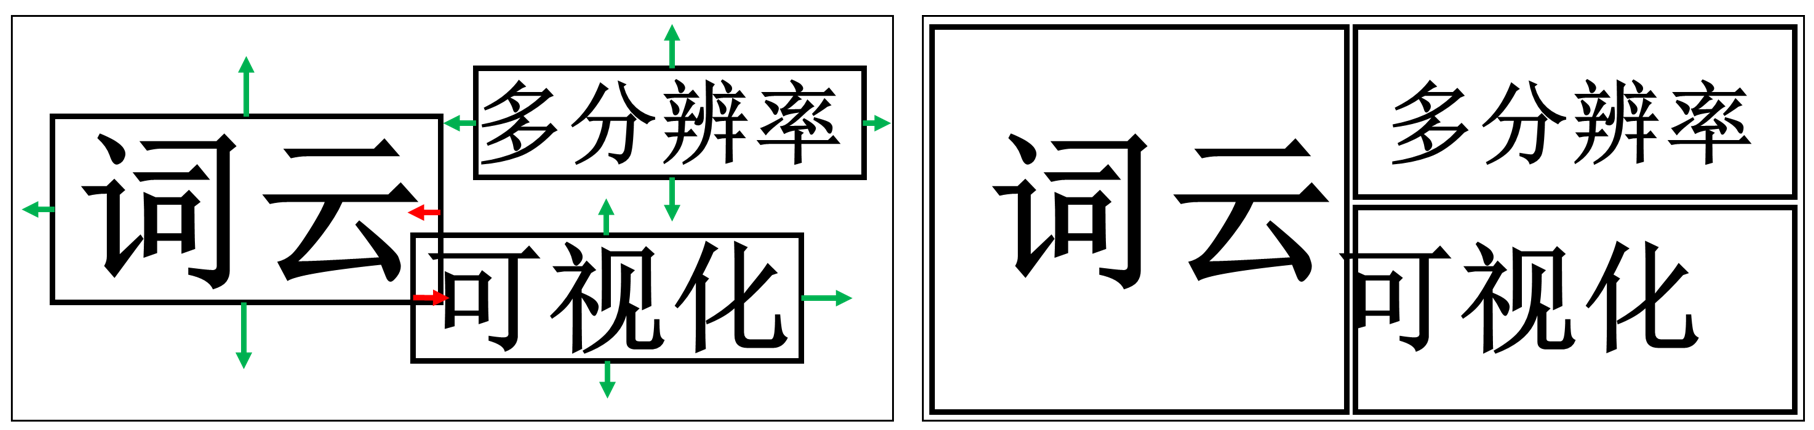
\includegraphics[width=\textwidth]{figures/expand.png}
	\caption{基于父文本布局的子文本区域分割算法示意图。左:原始父词云及其外接矩形,根据是否存在重叠得到各边扩张(绿)/收缩(红)的初始设定。右:经过逐步迭代后得到稳定的分割结果。}
	\label{fig:expand_alg}
\end{figure}

如图~\ref{fig:expand_alg}所示,我们的区域分割采用了一种基于迭代的策略。首先,从已知的父词云外接矩形出发,根据其四边是否与其他外接矩形相交判断其移动的方向---(1)若存在相交情况,则需要向内收缩,直至不存在交叠。(2)若不存在相交,则向外扩张,直至下一次遇到边界或产生相交。在接下来的每次迭代中,各个矩形的四边均向外或向内移动一个像素,除非其已满足停止的要求。记整个画布规格为$W\times H$,每一个词均对应于左上角坐标为$(x_0, y_0)$、右下角坐标为$(x_1, y_1)$的外接矩形,图~\ref{fig:collide_rule}左侧列举了在每一次迭代中需要对坐标对进行监测的情况以及边界的限制。按照定位坐标的相对位置,可将产生重叠的情况进一步分为边角重叠与区域包含与被包含三个状态。

所有区域满足终止条件时,能够严格保证每一个区域不交。但是,此时空白的地方有可能尚未被充分地利用。为此,我们再次对结果进行扫描,使用贪心的策略,依次对每个矩形区域的四边进行舒张。当伸展方向上不包含其他矩形时直接言延伸到画布边界;而当某些矩形存在于伸展方向上时,则选取距离待考察矩形最近的区域作为伸展的限制(见图~\ref{fig:collide_rule}右侧)。为了避免某些区域由于循环顺序优势伸展过多,我们将四个方位放于循环体外部。

\begin{figure}[htbp]
	\centering
	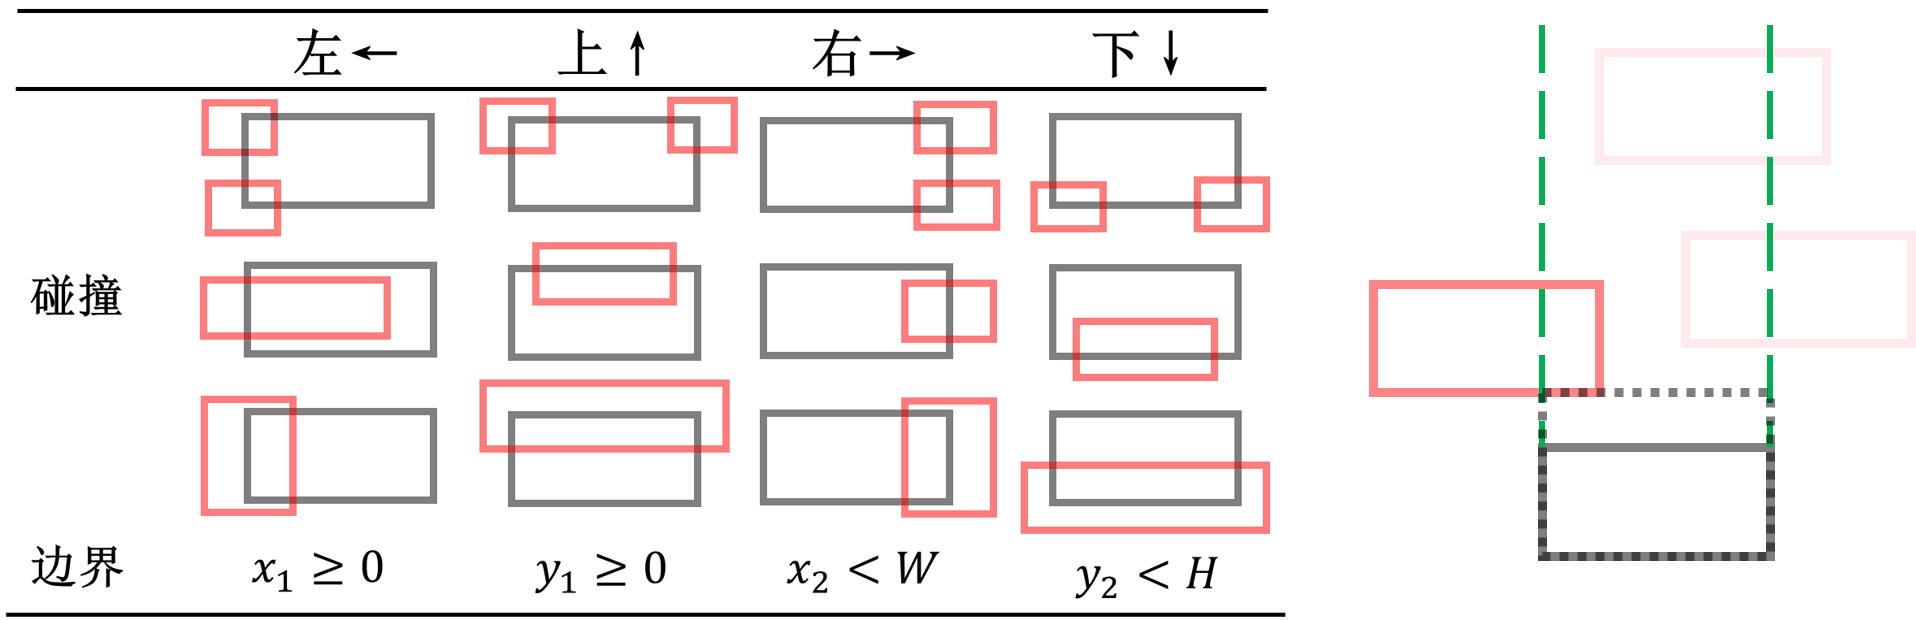
\includegraphics[width=\textwidth]{figures/collide_rule.png}
	\caption{左:子文本区域动态收缩/增长的监测规则与边界条件。黑色与红色矩形分别对应判断词云主体与相关区域。右:基于贪心策略的区域伸展策略。当黑色矩形需要向上伸展时,考察其上部在水平方向与其产生交叠的矩形区域,并基于距离最近矩形限制进行伸展。}
	\label{fig:collide_rule}
\end{figure}

\paragraph{分步布局}
获得子词云在画布上所对应的区域后,我们进一步考虑子词云的布局策略。若单纯随机布局,子词云与父词云之间会出现遮挡,不利于用户对文本的识别(P2.3)。为了充分利用可行区域(P2.1),我们在父词云实际所占区域的基础上,将子词云是否与其相交分为内外两层。内层子词云以父词云的轮廓作为边界,完全嵌套在父词云内部。而对于外层子词云,由于我们希望能稍加突出父词云的字形,我们使用父词云膨胀后取反的轮廓作为其布局的约束(见图~\ref{fig:sublayout})。
\begin{figure}[htbp]
	\centering
	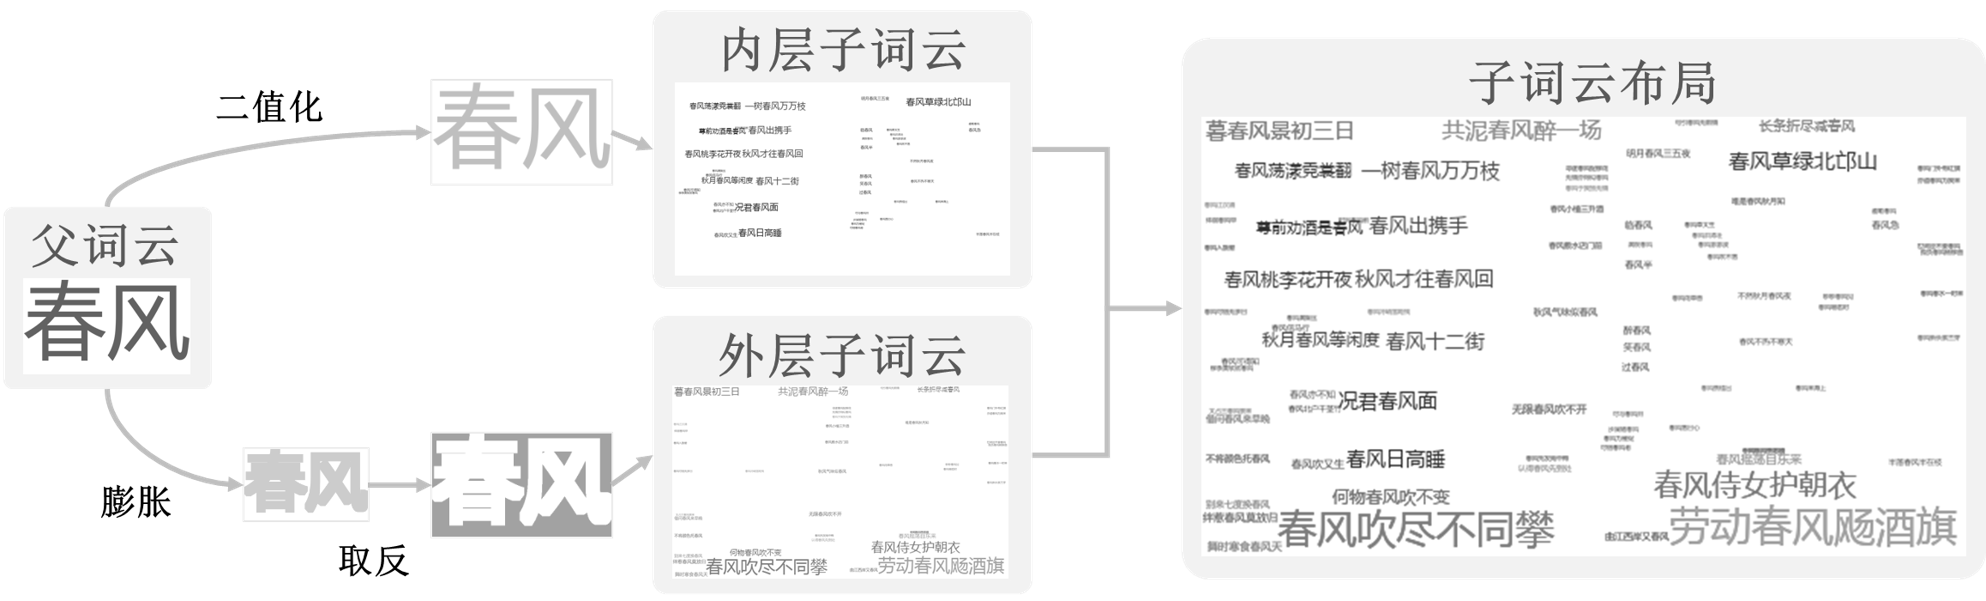
\includegraphics[width=\textwidth]{figures/sublayout.png}
	\caption{子词云分布布局的流程。首先以父文本构造布局约束,得到内层词云。再通过膨胀父文本结构后求反得到外层词云的布局约束,由此获得内层词云。}
	\label{fig:sublayout}
\end{figure}

膨胀的作用是一种常见的形态学处理方法,其作用是使二值图像中的物体沿轮廓向外扩大。设结构元$A$和集合$B$是$\mathbb{Z}^2$中的集合,则$A$对$B$的膨胀定义为
\begin{equation*}
A \oplus B = \{z|(\hat{B}_{z})\cap A = \varnothing\}.
\end{equation*}
此处我们设定结构元为以字符笔触宽度为边长的正方形,以此维护字体的原有形态。

\subsection{算法加速}
大屏上的双分辨率词云布局中最主要的问题就是分辨率过大,计算复杂。无论是使用何种算法,其复杂度都与画布尺寸相关,全屏情况即对应屏幕分辨率。由于无法避免检测词语位置是否重叠,基本上所有算法均需要对图像进行扫描,逐像素确定合适位置;而对于基于物理模拟的迭代算法如力导向布局,其计算更是代价高昂。因此,尽管以上的布局策略理论上可行,但在实际针对大屏的计算中,我们仍有一定的优化空间,提升算法效率。

首先,父文本词云的精确计算是不必要的。我们注意到,父文本词云具有相当大的字号,在远处浏览父词云的效果与在近处浏览常规词云的效果类似。换而言之,大屏上的父词云实际可视为整体放大的常规词云。因此,我们可以对父词云进行适当的全局放缩,在更小的画布上计算对应小字号词云的布局,再相应地映射到原有的大屏上,做一个简单的近似。

全局等比放缩系数$k$与父文本最小字号$m$有关。在设计选择的讨论中,我们已经确定父文本字号阈值设为$64$是合适的,而考虑到由于字号为离散整数,过度的放缩会限制词云字号的表示空间,也会产生过度失真的现象(见图~\ref{fig:font_size}),因此我们设定$16$像素为缩放后的最小字号,即$k = 64/16=4$。
\begin{figure}[htbp]
	\centering
	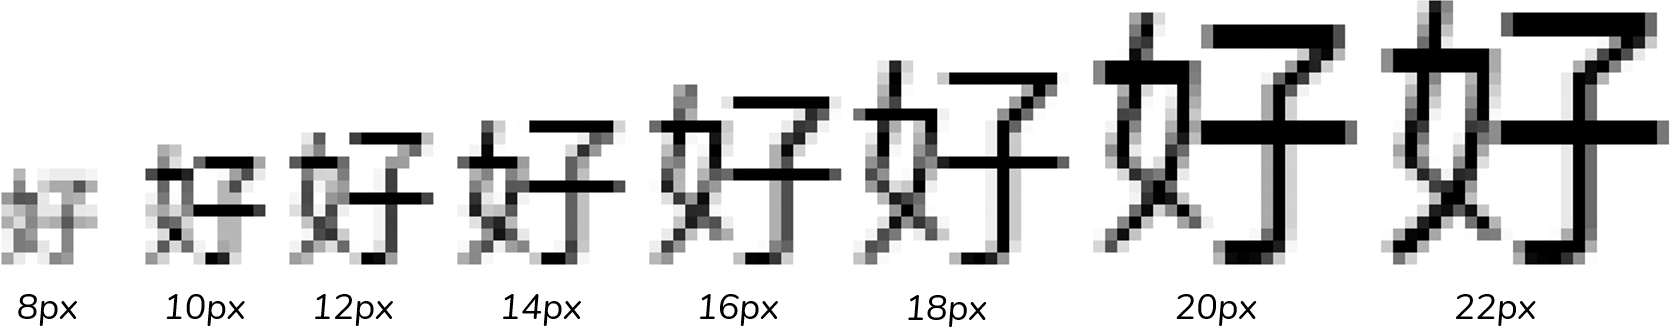
\includegraphics[width=0.8\textwidth]{figures/font_size.png}
	\caption{不同分辨率下的文字``好'',从左至右由10\texttt{px}至22\texttt{px}。分辨率越低,字形失真越严重。}
	\label{fig:font_size}
\end{figure}

例如,对一个由4$\times$3个4K显示屏所组成的大型显示设备,其具有$w_1\times h_1 = 15360\times6480$的分辨率。我们通过缩放,基于$w_2\times h_2 = 3840\times 1620$的画布尺寸得到每个词的基础坐标$\{(x_i', y_i')\}$。那么,经过一个线性变化,即可得到在原始画布上的布局坐标估计值:
\begin{equation*}
\begin{pmatrix}
x_i\\
y_i
\end{pmatrix}
 =  k\begin{pmatrix}
 x_i'-w_2/2\\
 y_i'-h_2/2
 \end{pmatrix}
 +\begin{pmatrix}
w_1/2\\
 h_1/2
 \end{pmatrix} .
\end{equation*}

其次,区域分割亦可在放缩后的画布上进行,减少搜索的空间。相关定位点的坐标转换可参考上式的横纵坐标转换。

最后,子词云布局算法可数据并行。由于在分割区域时已保证各子词云位置无重叠,因此各父文本对应的子文本词云的计算是完全独立的,可充分利用大型显示设备的GPU资源等来进行并行化计算,加速双分辨率词云生成的过程。

\section{混合图像}
我们在混合父词云与子词云时主要考虑了频域滤波以及词语颜色编码两个层面,以产生双分辨率的效果,同时保持父子词云在视觉上既相互关联又互不干扰。
\subsection{词云融合}
双分辨率词云的关键在于使人们在不同的距离下关注到不同层次的词云。参考Olivia等人~\supercite{Olivia2006}的多分辨率图像生成算法,我们同样采用先过滤父文本词云的高频分量,再通过透明度叠加的方法混合上下两个图层的方法来得到最终的结果(见图~\ref{fig:blend})。

\begin{figure}[htbp]
	\centering
	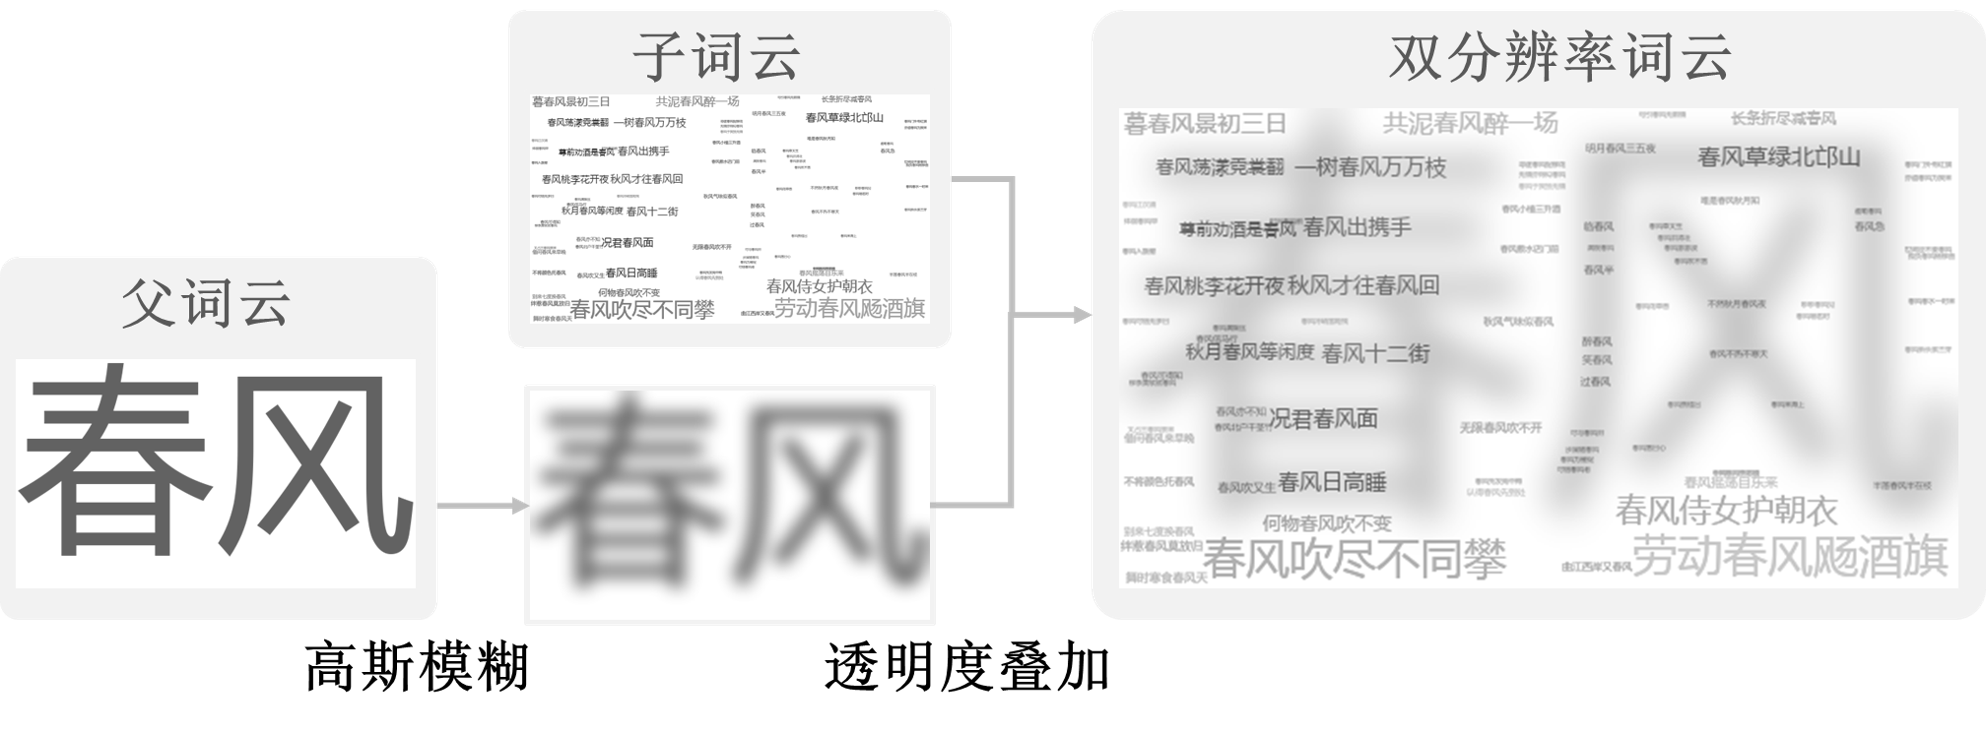
\includegraphics[width=\textwidth]{figures/blend.png}
	\caption{词云融合的流程图:保留父文本词云的高频分量,与子文本词云通过透明度互相叠加。}
	\label{fig:blend}
\end{figure}

由于子文本在双分辨率词云的设计中本就具有较小的字号,人们只有凑近屏幕至适宜阅读距离才能辨别,而滤波会影响其字形,因此我们不对其空间频域进行特殊处理。而对于字号较大的父文本,人们是从远处浏览,无需保留边界的细节即可辨认,且滤波后能够降低其对识别子词云产生的干扰,所以有必要过滤其高频分量。

简记在上一节所述布局算法得到的父文本词云为$I_1$,子文本词云为$I_2$。我们使用高斯滤波器对$I_1$进行卷积。一个标准的高斯函数$G(x,y)$的表达式为
\begin{equation*}
G(x,y) = \frac{1}{2\pi \sigma^2}e^{-\frac{x^2+y^2}{2\sigma^2}},
\end{equation*}
其中$\sigma$表示其标准差。一个高斯卷积核就是以核中心为原点的经过和归一化的离散高斯函数。
设$I_1$的最小字号为$s_{min} = \min_{i} s_i$,则我们限定高斯核$Ker(G)$的大小为$k^2 = ceil(\frac{s_{min}}{25})^2$。
\begin{equation*}
I_1' = I_1 \otimes Ker_k(G).
\end{equation*}
\begin{equation*}
I_2' = I_2.
\end{equation*}
$k$分母上的常数$25$是我们通过类似图~\ref{fig:font_size}的实验确定的,在常见的一些字体中,当分辨率$r$逐渐变大,对应字符比特图上的笔触宽度约为$ceil(\frac{r}{25})$。我们在全局使用与最小词云笔触大小一致的卷积核以防止字形剧变,影响识别。

经过$\alpha\in [0,1]\cap \mathbb{R}$的透明度叠加,最终得到的图像$I$可表示为
\begin{equation*}
I = \alpha I_1' + (1-\alpha)I_2'.
\end{equation*}


\subsection{颜色编码}

沿用设计选择C5,我们随机为父词云赋色,在此基础上对子词云添加扰动。但是,为了更加符合人的认知规律,我们选择在LCH色彩空间中进行相应的数值处理。

人是通过视网膜上分布的视杆细胞与视锥细胞来感知光线的,分别对应低亮度与高亮度的情况。Opponent-Process理论~\supercite{hurvich1957opponent}认为,大脑将感光细胞做感知到的光波处理为了三个通道——亮度、红绿与蓝黄通道。以此为理论指导,国际照明委员会定义了LAB色彩空间以模拟人的感知,经笛卡尔坐标系转换为圆柱坐标系后得到LCH色彩空间(见图~\ref{fig:color_rationale})。尽管彩色图片多以RGBA(分别对应红、绿、蓝、透明度)三个通道来编码一个像素所对应的颜色,使用RGB编码形式有利于计算机上的数字图像处理,但无论是基于RGB编码,亦或是可视化中常用的HSV/HSL编码,通过线性插值得到的渐变色并不能比拟于在HCL空间中所具有的渐变色依感知均匀分布的特性。
\begin{figure}[htbp]
	\centering
	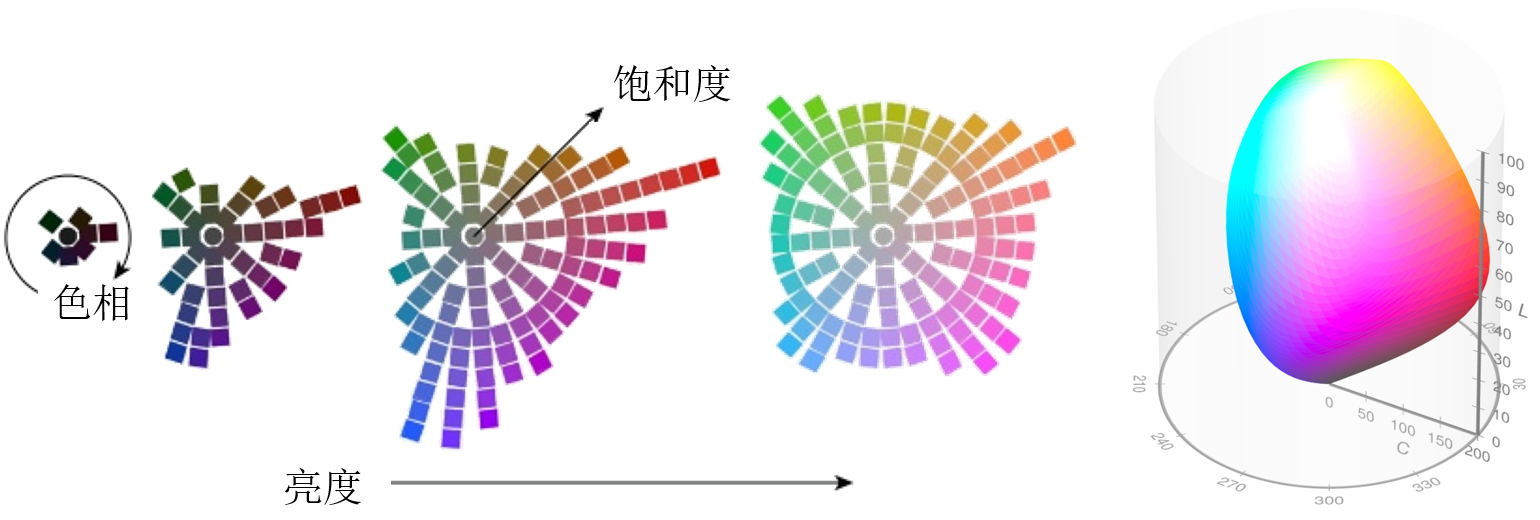
\includegraphics[width=0.9\textwidth]{figures/color_spec.png}
	\caption{色彩空间。左:不同亮度下人眼所能感知到的颜色示意(图源:NASA Earth Observatory\protect\footnotemark,标记经笔者翻译)。右:LCH色彩空间,分别对应亮度L、色度/饱和度C、与色相H(图源:维基百科\protect\footnotemark)。}
	\label{fig:color_rationale}
\end{figure}

\footnotetext{Subtleties of Color. Robert Simon. \url{https://earthobservatory.nasa.gov/blogs/elegantfigures/2013/08/05/subtleties-of-color-part-1-of-6/}}

\footnotetext{HCL color space. \url{https://en.wikipedia.org/wiki/HCL_color_space}}

在现有的普通词云布局算法中,颜色往往是独立于布局的,仅起到区分词语的作用。此时,这些算法会忽略透明度通道,直接随机取色或根据用户指定的一个配色方案在RGB空间中进行插值。对于具有语义聚类关系的词云,词云的色系将不同的类分别开,有时直接统一为同一颜色。而在双分辨词云中,经过一系列的测试与对比,我们设定了颜色编码规则如下,数值范围参考图~\ref{fig:color_rationale}右侧的色彩空间示意:

\begin{table}[htbp]
		 \caption{双分辨率词云色彩编码规则}
		 \label{tab:color_rule}
	\begin{tabular}{llll}

		\toprule
		&\multicolumn{1}{c}{父词云} & \multicolumn{1}{c}{相交子词云} & \multicolumn{1}{c}{不交子词云} \\
		\midrule
		亮度$L$ & 中等范围[$40,\  60$]    &   低亮度范围[$20,\  40$]     &    高亮度范围 [$60,\  80$]   \\
		色度$C$ &   中高色度范围 [$150,\  170$]  & 中色度范围[$120, \ 150$]     &  高色度范围 [$160,\  180$]       \\
		色相$H$ &  随机选择   &  父词云邻域 ±$10$°     &       父词云邻域  ±$10$°\\
		\bottomrule
	\end{tabular}
\vspace{-0.2cm}
\end{table}
在这一规则下,父词云区域与外部的子词云区域在亮度上具有较大的差异,但共享相同的色系,保证了在远处巨大的父词云清晰可辨(P2.3),并保留了父子词云的关联性。而在父词云的内部,同一色系但饱和度与亮度略低的子词云能够保证其不会完全混入父词云中,并能够强调父词云的字形。色彩的亮度实际上可以在背景色的基础上通过透明度来调节。但是,由于上下层词云混合时涉及到了基于透明度通道的图片叠加,为了减少不同参数对最终结果的关联性,我们在此并不考虑透明度。对于这样的规则,$\alpha$在$0.3\sim 0.5$的范围较为适宜(见图~\ref{fig:alpha_comparison})。
\vspace{-0.3cm}
\begin{figure}[htbp]
	\centering
	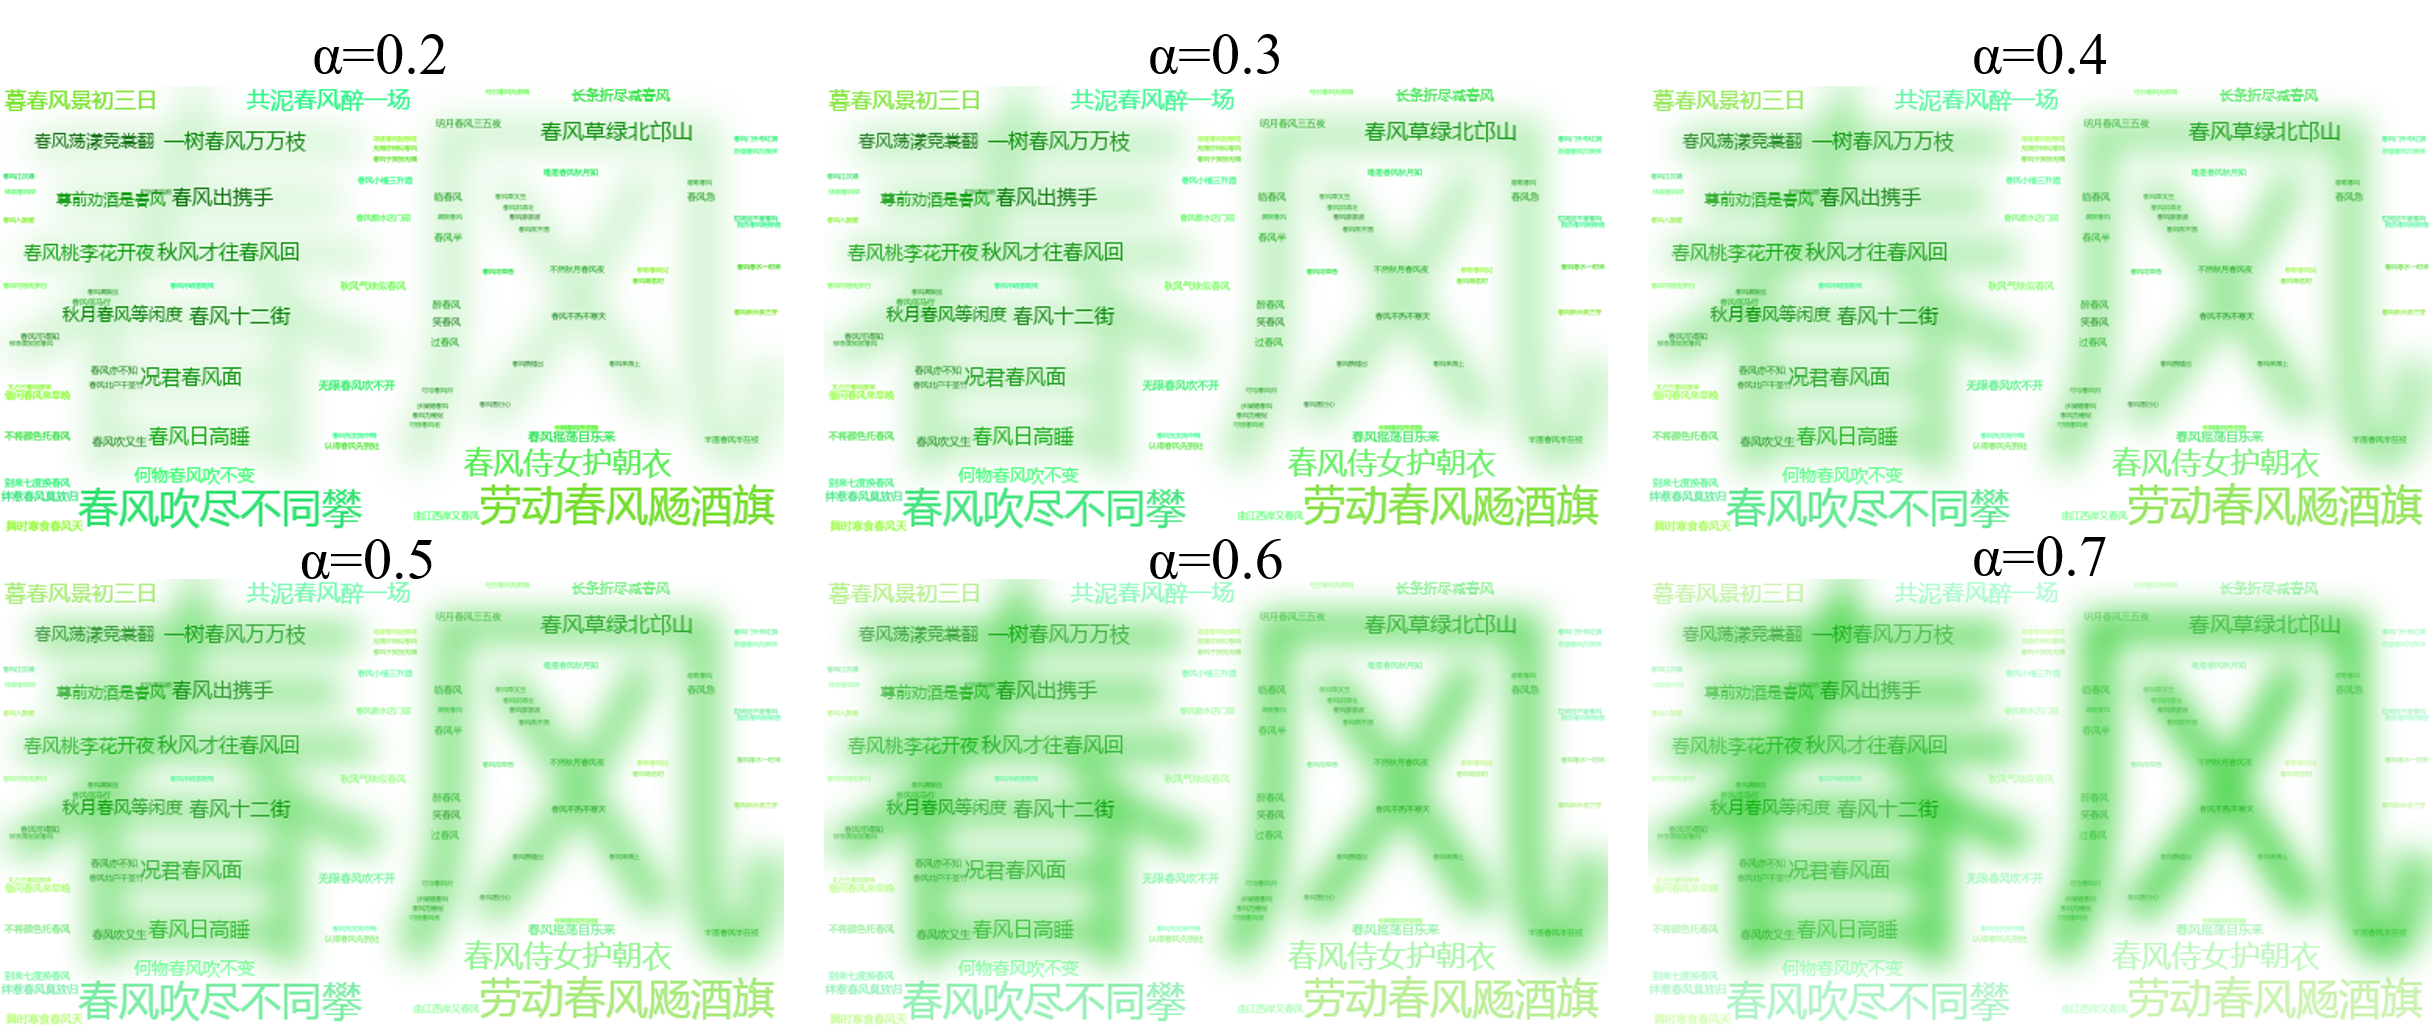
\includegraphics[width=\textwidth]{figures/alpha_comparison.png}
	\caption{不同$\alpha$值下的多分辨率词云效果。在表~\ref{tab:color_rule}的规则下,0.3至0.5为宜。}
	\label{fig:alpha_comparison}
\end{figure}
\vspace{-0.2cm}

图~\ref{fig:color_comparison}对比了在RGB编码下的随机扰动与基于上述LCH空间中的扰动策略。可以观察到,尽管由于透明度叠加的原因,靠近屏幕时两种方法对应的子词云均清晰可辨;但当我们远离屏幕,LCH编码策略下外层词云总体偏亮的色彩能让我们更为轻松地辨认出父词云的字,而相对而言,RGB随机编码产生的图片稍显噪音过多。
\vspace{-0.1cm}
\begin{figure}[htbp]
	\centering
	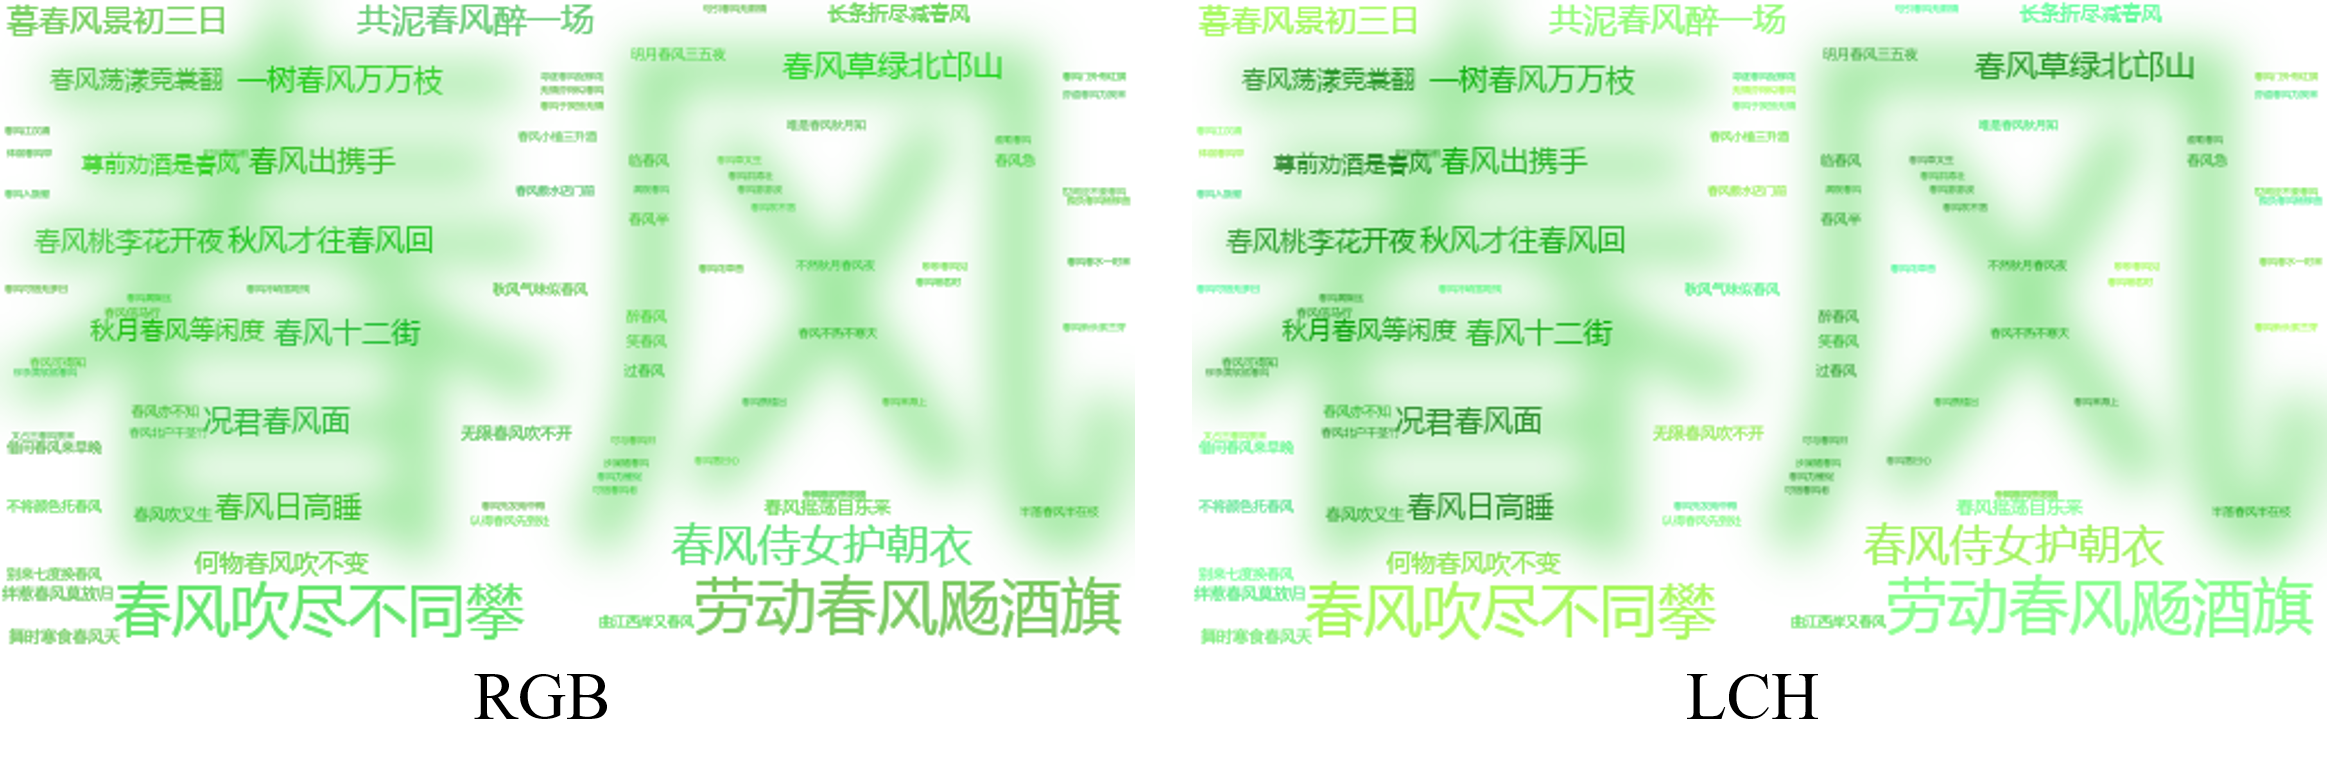
\includegraphics[width=\textwidth]{figures/color_comparison.png}
	\vspace{-0.5cm}
	\caption{子词云颜色编码策略对比。左:基于RGB空间的扰动。右:基于LCH空间的扰动。}
		\vspace{-0.5cm}
	\label{fig:color_comparison}
\end{figure}
